\chapter{Hardware Implementation} \label{chap:hardware}
This chapter describes the practical implementation of the system on the physical hexapod robot. Section  \ref{sec:hardware_overview} provides an overview of the implementation. Section \ref{sec:ros_nodes} describes the \ac{ros} in the system, their functions and the data they communicate. Appendix \ref{app:ros_comms} describes the details of the \ac{ros} messages sent by the nodes and their data types.

\section{Overview} \label{sec:hardware_overview}
The entire system was implemented in the \acf{ros} environment, \ac{ros} is a system which, among other things, greatly simplifies the task of communication between devices using various different communication protocols. This is achieved by sectioning all code into different \ac{ros} nodes, where every node is treated as a component in a large network. All ros nodes are joined together by the core node, which is hosted at a set IP address on the network.

\section{ROS Architecture} \label{sec:ros_nodes}
    \ac{ros} operates by the concept of nodes, publishers and subscribers. A \ac{ros} node is a piece of code executed in the \ac{ros} network, publishers and subscribers are initialised by a node. A publisher will send a message into the \ac{ros} network, while a subscriber will listen for a certain message on the network. When a subscriber receives a message it will execute a user defined callback function to use the received data.

    The various \ac{ros} nodes are distributed between the base station on the desktop computer, and the Jetson Nano and the Teensy \ac{mcu} on the hexapod robot. Figure \ref{fig:nodes} provides an overview of the nodes and how they communicate with each other.

    \captionsetup[figure]{oneside,margin={0cm,0cm}}
    \begin{figure}[h]
        \centering
        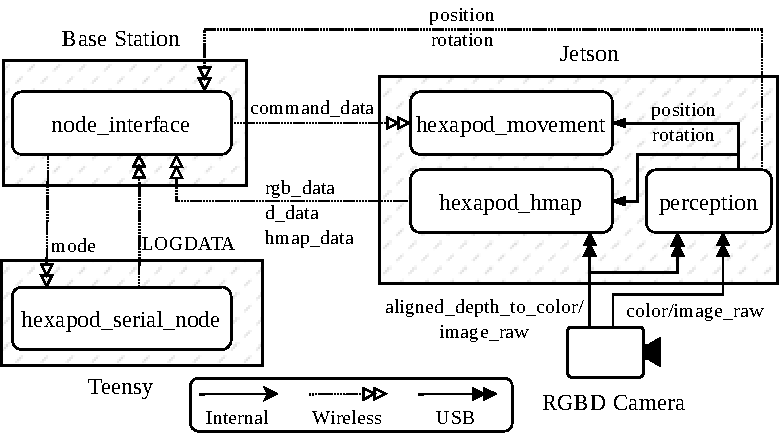
\includegraphics{Diagrams-Nodes.drawio.pdf}
        \caption{ROS nodes and communication.}
        \label{fig:nodes}
    \end{figure}

    \noindent
    Note that the data transfer arrows between the base station and the teensy are a combination of the wireless and USB arrows, this implies that the data passes to the Jetson as a intermediate step. Transfers between the base station and the Jetson are wireless, while between the Jetson and the Teensy are through USB. Section \ref{sec:base_ros} and \ref{sec:on_board_ros} provide details on the node architecture shown in figure \ref{fig:nodes}.
    \subsection{Base Station} \label{sec:base_ros}
        The base station consists of a single \ac{ros} node, this node is responsible for transmitting all commands to and receiving data from the robot. The base station publishes two messages, the mode message and the command data message. As the names imply the mode message contains the commanded mode that the robot should switch to, while the command data message contains the remaining commands that the operator could issue. The mode is separated from the other commands because it is only sent to the Teensy, while the other commands are sent to the Jetson.
        
        The base station subscribes to the pose message from the perception node, and the rgb data, d data and hmap data from the hexapod map node, and also the LOGDATA message from the hexapod serial node. The pose message contains the pose estimate produced from ORB-SLAM3, while the rgb data, d data and hmap data message contain the color, depth and heightmap images respectively. The LOGDATA message contains generic string log messages from the Teensy.
        
        The base station is what the operator uses to observe and issue commands to the robot, as such there is wireless communication link between the robot and the base station.
        % For a description of the base station publishers see table \ref{tab:base_pubs} and for its subscribers see \ref{tab:base_subs}. Table \ref{tab:data_types} describes
        % data types used.
        % \begin{table}[h]
        %     \centering
        %     \begin{tabularx}{\textwidth}{| l | l | X | l |}
        %         \hline
        %         \multicolumn{4}{|c|}{\textbf{Base Station Publishers}} \\ \hline
        %         \textbf{Name} & \textbf{Data Type} & \textbf{Description} & \textbf{Frequency} \\ \hline
        %         % walk\_dir & Description & Data Type & Frequency \\ \hline
        %         command\_data & HexapodCommands & Various robot command parameters. & On change \\ \hline
        %         mode & Int32 & Specifies the oporationg mode of the robot. & On change. \\ \hline
        %     \end{tabularx}
        %     \caption{Base station publishers}
        %     \label{tab:base_pubs}
        % \end{table}
        Among the commands the operator can send the robot is the operating mode, the robot currently only has two operating modes, torque cutoff mode and walking mode. The torque cutoff mode is the initial mode the robot is in, while in this mode the leg servos disable all torque control, thus entering a relaxed state. In walking mode the robot walks in the commanded direction whilst optimising its foot positions according to the terrain. If the robot encounters a piece of terrain for which no optimisation can be found the human controller will have to adjust the walking direction from the base station.

        % \begin{table}[h]
        %     \centering
        %     \begin{tabularx}{\textwidth}{| l | l | X |}
        %         \hline
        %         \multicolumn{3}{|c|}{\textbf{Base Station Subscribers}} \\ \hline
        %         \textbf{Name} & \textbf{Data Type} & \textbf{Description} \\ \hline
        %         % walk\_dir & Description & Data Type & Frequency \\ \hline
        %         rgb\_data & Image & The processed color image from the robot. \\ \hline
        %         d\_data & Image & The processed color depth from the robot. \\ \hline
        %         hmap\_data & Image & The heightmap generated on the robot. \\ \hline
        %         LOGDATA & String & General logs from the robot. \\ \hline
        %     \end{tabularx}
        %     \caption{Base station subscribers}
        %     \label{tab:base_subs}
        % \end{table}
        
        % \noindent
        % The only subscribers present on the base station are the processed camera images, heightmap and logs. These are all used to provide a interface from where
        % the operator can control the robot.

    \subsection{On Board} \label{sec:on_board_ros}
        The hexapod has two computational units on board, first the Jetson Nano, which handles all high level operations, including heightmap generation and scoring, foot optimisation, maintain a walking gait and localisation using ORB-SLAM3. Secondly a Teensy2.0 \ac{mcu} handles low level operations, including interpolating feet movement paths and servo control.

        The Jetson hosts four different nodes, the hexapod hmap, hexapod movement, RGBDSLAM and rs camera nodes. The rs camera node publishes the camera stream consisting of the color and aligned depth to color messages. As could be deduced from the names, the depth message is aligned to the color. These messages are transmitted at a rate of 30Hz.
        
        The RGBDSLAM module runs the ORB-SLAM3 algorithm and subscribes to the depth and color streams from the rs camera node as inputs. As ORB-SLAM3 uses both the color and depth streams for pose estimation these streams are synchronised in time. Once the pose is estimated it is published in the pose message.

        The hexapod hmap node is responsible for generating the heightmap and score maps. It subscribes to the pose, depth and color messages, the depth and color messages are downsampled before being used to generate the heightmap. The entire generation process is ran on the Jetson Nano's \ac{gpu} as described in chapter \ref{chap:mapping}. Once the heightmap and scoremap are generated they are published in the hmap data and scoremap data messages. Additionally the downsampled colour and depth messages are also published for transmission to the base station.

        Next, the hexapod movement node subscribes to the command, pose, hmap and scoremap messages to generate and optimise the feet targets, as described in chapter \ref{chap:motion} and \ref{chap:optimisation}. The feet targets are published as the effector targets message.

        Lastly, the Teensy \ac{mcu} also consists of a single \ac{ros} node, the hexapod serial node. The functionality of this node is simply to facilitate communication over USB. The node is subscribed to the mode and effector targets messages, these messages are then used to calculate the feet trajectories as described in chapter \ref{chap:motion}. The trajectories are then translated into servo angles and angular rates, also described in chapter \ref{chap:motion}. Whereafter the servos are actuated. The only publisher present on the Teensy is the LOGDATA publisher, which simply publishes general string log messages for use by the operator.
    %     Table \ref{tab:jetson_pubs} to \ref{tab:teensy_subs} describe the \ac{ros} publishers and subscribers present on these two computational units.
        
    %     The camera data, heightmap data, position and rotation are published for display at the base station.
    %     While the effector targets are published for use on the Teensy to move the robot's feet to the optimised positions.
    %     \newpage
    %     \begin{table}[h]
    %         \centering
    %         \begin{tabularx}{\textwidth}{| l | l | X | l |}
    %             \hline
    %             \multicolumn{4}{|c|}{\textbf{Jetson Publishers}} \\ \hline
    %             \textbf{Name} & \textbf{Data Type} & \textbf{Description} & \textbf{Frequency} \\ \hline
    %             % walk\_dir & Description & Data Type & Frequency \\ \hline
    %             effector\_targets & EffectorTargets & Data indicating which feet to move where, and what type of interpolation to use. & On change\\ \hline
    %             rgb\_data & Image & The processed color image from the \ac{rgbd} camera. & 15Hz. \\ \hline
    %             d\_data & Image & The processed depth image from the \ac{rgbd} camera. & 15Hz. \\ \hline
    %             hmap\_data & Image & The heightmap generated on the robot. & 15Hz. \\ \hline
    %             position & Vector3 & The localised position of the robot & 15Hz \\ \hline
    %             rotation & Quat & The localised rotation of the robot & 15Hz \\ \hline
    %         \end{tabularx}
    %         \caption{Jetson publishers}
    %         \label{tab:jetson_pubs}
    %     \end{table}
    %     % \newpage
    %     \begin{table}[h]
    %         \centering
    %         \begin{tabularx}{\textwidth}{| l | l | X |}
    %             \hline
    %             \multicolumn{3}{|c|}{\textbf{Jetson Subscribers}} \\ \hline
    %             \textbf{Name}  & \textbf{Data Type} & \textbf{Description} \\ \hline
    %             % walk\_dir & Description & Data Type & Frequency \\ \hline
    %             command\_data & HexapodCommands & Operator commands. \\ \hline
    %             color/image\_raw & Image & Color image from the camera. \\ \hline
    %             aligned\_depth\_to\_color/image\_raw & Image & Depth image from the camera. \\ \hline
    %         \end{tabularx}
    %         \caption{Jetson subscribers}
    %         \label{tab:jetson_subs}
    %     \end{table}

    %     As can be seen from table \ref{tab:jetson_subs} the only subscribers required on the Jetson is the raw camera feed, 
    %     for constructing the heightmap, and the commands from the base station.

    %     Table \ref{tab:teensy_pubs} show that the Teensy publishes the current feet positions these are the positions calculated through \ac{fk}. Additionally
    %     log data is also published for use on the base station.
    %     \begin{table}[h]
    %         \begin{tabularx}{\textwidth}{| l | l | X | l |}
    %             \hline
    %             \multicolumn{4}{|c|}{\textbf{Teensy Publishers}} \\ \hline
    %             \textbf{Name} & \textbf{Data Type} & \textbf{Description} & \textbf{Frequency} \\ \hline
    %             LOGDATA & String & General logs. & 10Hz \\ \hline
    %             effector\_current\_position & Eigen::Vector3d & Current feet positions. & 10Hz \\ \hline
    %         \end{tabularx}
    %         \caption{Teensy publishers}
    %         \label{tab:teensy_pubs}
    %     \end{table}
    %     \begin{table}[h]
    %         \centering
    %         \begin{tabularx}{\textwidth}{| l | l | X |}
    %             \hline
    %             \multicolumn{3}{|c|}{\textbf{Teensy subscribers}} \\ \hline
    %             \textbf{Name} & \textbf{Data Type} & \textbf{Description} \\ \hline
    %             % walk\_dir & Description & Data Type & Frequency \\ \hline
    %             command\_data & HexapodCommands & The color image from the \ac{rgbd} camera. \\ \hline
    %             effector\_targets & EffectorTargets & Data indicating which feet to move where, and what type of interpolation to use.\\ \hline
    %             mode & Int32 & Receives mode data from the base station \\ \hline
    %         \end{tabularx}
    %         \caption{Teensy subscribers}
    %         \label{tab:teensy_subs}
    %     \end{table}

    %     Lastly, from table \ref{tab:teensy_subs} it can be seen that the Teensy subscribes to the command data, effector targets and mode.
    %     The walking speed component from the command data is used to set the rotational rate of the servos, as discussed in section \ref{sec:ang_rate}.
    %     The effector targets are used to interpolate a curve for the feet to move along, as described in section \ref{sec:arc_generation}. The mode is required
    %     as some modes could integrate directly with the servo control, namely the torque cutoff mode.

    % \newpage
    % \subsection{ROS Data Types}
    %     Various custom \ac{ros} data types are defined to assist with communication, these data types are described in table \ref{tab:data_types}.
    %     \begin{table}[h]
    %         \centering
    %         \begin{tabularx}{\textwidth}{| l | p{\widthof{float32\([2]\) walk\_dir}} | X |}
    %             \hline
    %             \textbf{Name} & \textbf{Type Definition} & \textbf{Description} \\ \hline
    %             % walk\_dir & Description & Data Type & Frequency \\ \hline
    %             Vector3 & float\([3]\) data. & A vector in 3D space.  \\
    %             \hline
    %             EffectorTargets & Vector3\([6]\) targets \newline 
    %                             bool\([6]\) swinging. & Data describing the targets of the robot's feet and which feet are swinging. \\
    %             \hline
    %             HexapodCommands & float32\([2]\) walk\_dir \newline
    %                             float32 speed \newline
    %                             float32 height & Data packet containing various command parameters for the robot. \\
    %             \hline
    %         \end{tabularx}
    %         \caption{\ac{ros} data type descriptions}
    %         \label{tab:data_types}
    %     \end{table}